% conceptualisation of signature detection
    % small unit
    % complex descirption (F&F)
    % cluster analysis
The method of identification of spatial signatures consists of three top-level steps.
First, we delineate a spatial unit of analysis that reflects the structure of
urban phenomena on a very granular level. Then we characterise each of them
according to form and function, capturing the nature of each unit and its spatial
context. Finally, we use cluster analysis to derive a typology of our spatial units
that, once combined into contiguous areas, forms a typology of spatial signatures.

\subsection*{Spatial unit}
% spatial unit
    % conceptualisation of enclosed tessellation
    % rules
        % indivisible
        % internally consistent
        % geographically exhaustive
    % options
        % admin boundaries
        % arbitrary grids
        % morphological units
    % ET design
        % barriers
        % enclosures
        % anchors
        % ET cells
The first major methodological decision relates to the definition of the
spatial unit. An ideal candidate needs to reflect space in a granular manner, and we argue
it should fulfil three conditions. First, it should be \textit{indivisible},
meaning that any subdivision would result in a unit that is incapable of
capturing the nature of urban form and function. Second, it needs to be
\textit{internally consistent} - it should always reflect only a single signature type.
Last, it should be geographically \textit{exhaustive}, covering the entirety of the study
area.

Spatial units used in literature can be split into three groups. One is using
administrative boundaries like city regions\cite{angel2020}, wards or census output areas\cite{alexiou2016}, that are
convenient to obtain and can be easily linked to auxiliary data. However,
those rarely reflect the morphological composition of urban space and, in some cases, may
even “obscure morphologic reality”\cite{taubenbock2019new}. At the same time, most of them
are divisible, and larger units are not always internally consistent. Another group is based on
arbitrary uniform grids linked either to spatial indexing methods like
H3\cite{brodsky2018h3} or Ordnance Survey
National Grid, or to ancillary data of remote sensing or other origins like a
WorldPop grid\cite{jochem2021tools}. Grids however cannot be considered internally
consistent as
they do not consider the underlying structure of the landscape.
Finally, urban morphology studies tend to use morphological elements as
street segments\cite{araldi2019}, blocks\cite{gil2012},
buildings\cite{hamaina2012a} or plots\cite{bobkova2019} as units of analysis.
Some of those
could be seen as indivisible and internally consistent, but since they are largely based
on built-up fabric, they are not exhaustive. For example, in areas without any building or
street, there
is no spatial unit to work with. Plots could be theoretically considered as exhaustive,
consistent and indivisible, but there is no accepted conceptual definition and unified
geometric representation\cite{kropf2018}.

We are, therefore, proposing an application of an alternative spatial unit called \textit{enclosed
tessellation cell} (ETC), defined as "the portion of space that results
from growing a morphological tessellation within an enclosure delineated by a series
of natural or built barriers identified from the literature on urban form, function and
perception"\cite{dab_mf_2021a}.
% We should drop a reference to the conceptual paper here.
ETCs follow the morphological tradition in that it is
based on the physical elements of an environment but overcome the drawbacks of
conventionally used units. Its geometry is generated in the three steps illustrated on a
Figure \ref{fig:et_diagram}. First, a set of features representing physical barriers
subdividing space, in our case composed of the street network, railways, rivers and a
coastline, is combined, generating a layer of boundaries (\ref{fig:et_diagram} A).
These then partition space
into smaller enclosed geometries called \textit{enclosures} (\ref{fig:et_diagram} B),
which can be very granular
or very coarse depending on the geographic context. In dense city centres where a single
enclosure represents a single block is a high frequency of small enclosures. At the same time, in the
countryside, this approach leads to very few large enclosures as their delimiters are far away
from each other. Enclosures are then combined with building footprints (\ref{fig:et_diagram} B),
which act as
anchors in space and potentially subdivide enclosures into enclosed tessellation cells using the
morphological tessellation algorithm\cite{fleischmann2020} (\ref{fig:et_diagram} D),
a polygon-based adaptation of Voronoi
tessellation. The resulting geometries are indivisible as they contain, at most, a single
anchor building, internally consistent due to their granularity and link to morphological
elements composing urban fabric, and geographically exhaustive as they cover an entire area
limited by specified boundaries.

\begin{figure}
    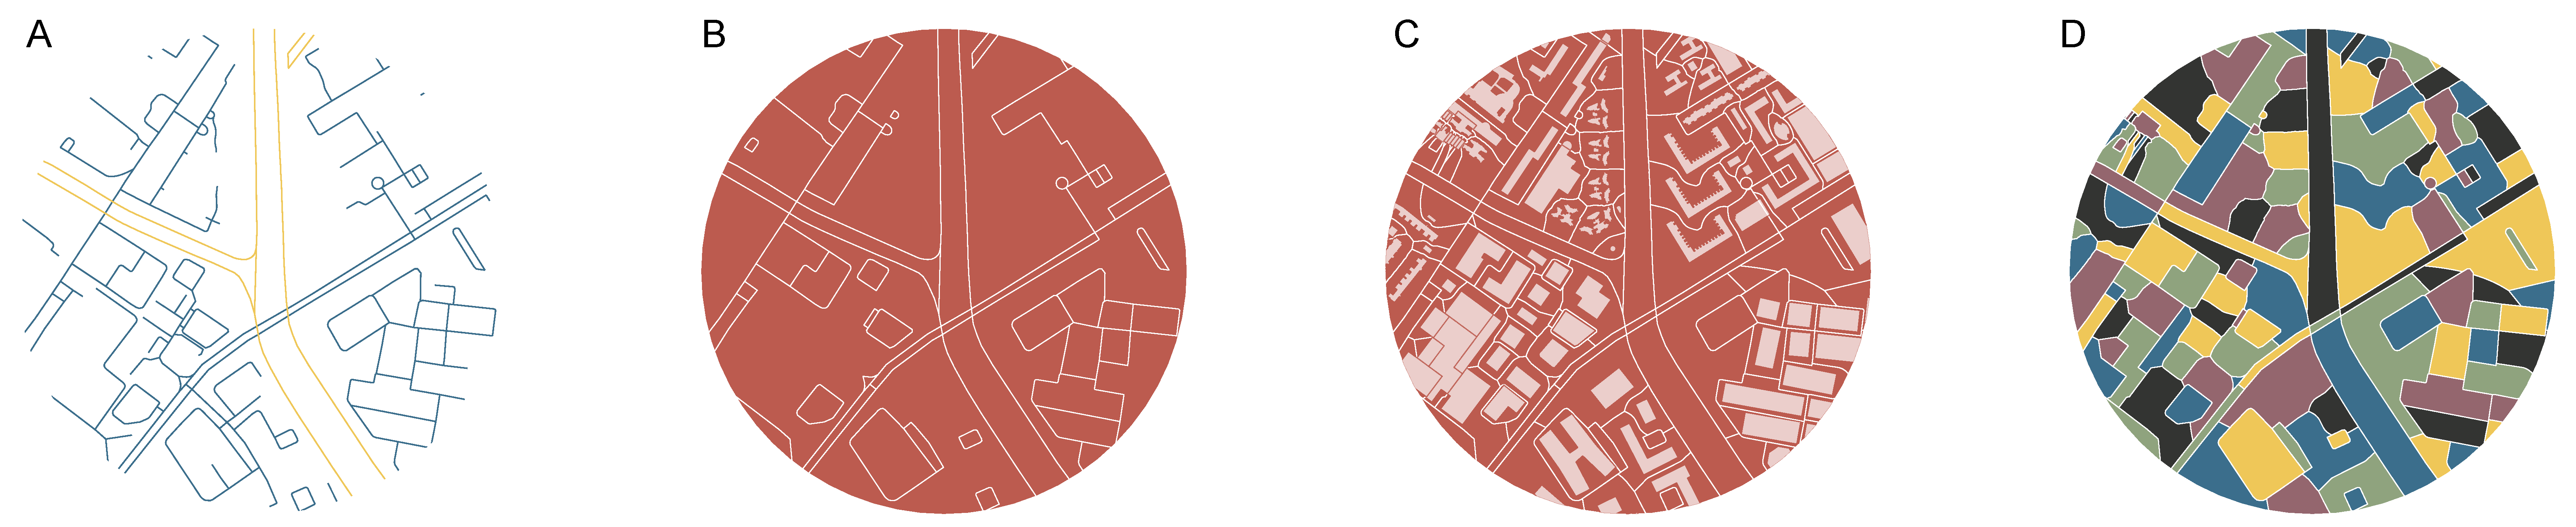
\includegraphics[width=\linewidth]{fig/et_diagram.pdf}
    \caption{Diagram illustrating the sequential steps leading to the delineation of
    enclosed tessellation. From a series of enclosing components, where blue are streets
    and yellow river banks (A), to enclosures (B), incorporation of buildings as anchors
    (C) to final tessellation cells (D).}
    \label{fig:et_diagram}
\end{figure}

    % data input
        % barries
            % roads from OS Open Roads
                % data description (simplified centerlines)
            % railway from OS OpenMap - Local
                % data description (simplified centerlines)
            % rivers from OS OpenRivers
                % data description (simplified centerlines)
            % coastline from OS Strategi®
                % data description (continuous enclosing geometry)
        % buildings
            % OS OpenMap - Local
            % data quality description (merged adjacent geometries)

In our ODP for Great Britain, street networks are extracted from OS
Open Roads datasets\cite{openroads2020} representing simplified road centrelines
cleaned of underground road segments.
Railways are retrieved from OS OpenMap - Local\cite{openmap2020}
("RailwayTrack" layer) which captures surface railway tracks. Rivers are extracted from
OS OpenRivers\cite{openrivers2020} representing river network of GB as centrelines, and a coastline is
retrieved from OS Strategi®\cite{strategi2016}, capturing coastline as a continuous line
geometry. Building geometry is extracted, again, from OS OpenMap - Local ("Building"
layer) and represents generalised building footprint polygons.\footnote{Note that the dataset
does not distinguish between individual buildings when they are adjacent (e.g. perimeter
block composed of multiple buildings is represented by a single polygon).}

% characterisation of space
\subsection*{Characterisation of space}
Spatial signatures capture the character of the built and unbuilt environment
based on two components - form and function. Each of them is quantified at the level of
individual ETCs using methods appropriate for each specific dataset. While form
is described using urban morphometrics (i.e. quantitative analysis of urban
form)\cite{dibble2019origin}, function is a composite of a variety of data inputs. We outline each
component with a bit more detail below.

\subsubsection*{Form}
    % form
        % input data
            % ET cells
            % bulidings
            % street network
        % morphometrics
            % different categories of characters
                % dimension
                % shape
                % spatial distribution
                % intensity
                % connectivity
                % diversity
            % different scales
                % individual elements -> adjacency -> networks
        % contextualisation
            % interest in characterisation of spatial patterns
            % distance-weighted higher order contiguity spatial weights
            % reflection of a statistical distribution of data within context
                % proxy of diversity
Morphometric characterisation of urban form is based on the numerical description
of four elements capturing the built environment - buildings, streets, ETCs, and
enclosures - and reflects their patterns based on six categories of
characters: dimensions, shapes, spatial
distribution, intensity, connectivity and diversity\cite{fleischmann2020a}. Each element is considered across
different scales, from the measurement of individual geometries, to relations of
neighbouring geometries, to a graph-based analysis of the street network. The combination of
elements, categories and scales results in a set of 59 individual morphometric
characters listed in the online table 1.

% Q: do we want to include some morphometric theory here? I'd say no since this is a
% data descriptor but I can add some if needed.

However, measuring individual characters is not enough to understand the predominant
spatial patterns. For some types of urban form, high heterogeneity is not
uncommon. This means that using, for example, areas of building footprints would, in most cases, result
in largely discontinuous clusters that do not capture the aspect of an area. Therefore, we represent each of the
morphometric characters using three summary variables reflecting statistical distributions
of measured data within a spatial context of each ETC. Context is defined as
tenth
order of contiguity computed across the mesh composed of contiguous ETCs. Furthermore, each
value is weighted by the inverse distance between so-called poles of inaccessibility
(defined as a centre of a maximum inscribed circle) of each ETC. Three proxy variables
then capture the first, the second and the third quartile of the resulting weighted
distribution. Such a characterisation can capture the contextual tendency of each
morphometric character and hence identify contiguous clusters in both homogenous and
heterogeneous urban tissues.

\subsubsection*{Function}
    % function
        % input data
            % overview - from population and POIs to NDVI and night lights
            % include table with transfer methods
        % transfer methods overview
            % blg-based interpolation
            % areal interpolation
            % accessibility
            % euclidean distance
            % zonal statistics
        % contextualisation
            % depending on the transfer method, function-based characters we
            %  contextualised using the same method used in morphometrics
Characterisation of the function component uses a different approach. While data
describing urban form are not generally available in a processed format, forcing us to employ morphometric approaches, different aspects of function are often available as
open data products. Therefore, the main goal of our characterisation of ETCs based on
function is to develop appropriate transfer methods to link data published as grids or
linked to administrative boundaries to ETCs.

In this work, we are using five different transfer methods: Areal interpolation,
Building-based dasymetric areal interpolation\cite{eli_knaap_2021_5047613}, Network-constrained accessibility,
Euclidean accessibility, and Zonal statistics. Areal interpolation is used when the
functional data covers the entirety of space in the
form of polygon geometry and when there is no assumption that the phenomena it captures
are linked directly to the human population, such as land cover data. When there is
an assumption of relation to the population, building-based dasymetric areal
interpolation is used instead. The main difference is that instead of ETC polygons,
building footprint polygons linked to individual ETCs are used as a target of
interpolation. That ensures that data like population estimates are linked to ETCs
proportionally to their ability to house population rather than by their area.
Network-constrained accessibility is used when the input data represent points of
interest like locations of supermarkets. Points are then snapped to the nearest node on
the street network and linked to the ETCs through the count of observations
accessible from the cell within 15 minutes of walk (1200m on the street network) and a distance to the nearest point. In
some cases, Euclidean (as-crow-flies) accessibility is measured instead to accommodate
for phenomena that are often outside the reach of a drivable network like water bodies.
Zonal statistics are used to transfer data originally stored in a raster
format to ETCs as the mean value of raster pixels intersecting each polygon
geometry. Finally, characters based on interpolation and zonal statistics are expressed
using their contextual versions following the method used for form characters to, again,
reflect the contextual pattern of measured values. The selection of datasets and the chosen
transfer method are listed in the table \ref{tab:function}.

\begin{table}
\begin{tabular}{p{35mm}p{50mm}p{35mm}p{40mm}}
\toprule
                                data & source &                   input geometry &                               transfer method \\
\midrule
                Population estimates & ONS Census Output Area population estimates, Statistics.gov.scot &     Vector (output area polygon) & Building-based dasymetric areal interpolation \\
          Retail POIs (supermarkets) & Geolytix &                   Vector (point) &             Network-constrained accessibility \\
                        Water bodies & OS OpenMap Local &      Vector (water body polygon) &                       Euclidean accessibility \\
                    Listed Buildings & Historic England, Historic Environment Scotland, Lle Geo-Portal for Wales &                   Vector (point) & Network-constrained accessibility \\
                        Night Lights & VIIRS DNB Nighttime Lights &                    Raster (500m) &                              Zonal statistics \\
  Food Hygiene Rating Scheme Ratings & CDRC.ac.uk &                   Vector (point) &             Network-constrained accessibility \\
                Workplace population & ONS Census Workplace population, Scotland's census Workplace population &     Vector (output area polygon) & Building-based dasymetric areal interpolation \\
         Culture (theatres, cinemas) & OpenStreetMap &                   Vector (point) &             Network-constrained accessibility \\
                   Corine land cover & Copernicus Land Monitoring Service & Vector (land cover zone polygon) &                           Areal interpolation \\
                                NDVI & GHS-composite-S2 R2020A &                     Raster (10m) &                              Zonal statistics \\
                      Retail centres & CDRC.ac.uk &   Vector (retail centre polygon) &                       Euclidean accessibility \\
\bottomrule
\end{tabular}

\caption{\label{tab:function}Functional characters used to
describe the function component of spatial signatures. For details of the implementation,
refer to the reproducible Jupyter notebooks available at urbangrammarai.github.io.}
\end{table}

\subsection*{Cluster analysis}
% cluster analysis
    % comparison of clustering methods (shall we include this?? skip for now, keep only
    % as a notebook online)
        % K-Means, GMM, SOM

    % two levels of K-Means clustering
        % data input
            % combination of both form and function, all characters equally weighted
            % only contextualised representation of characters is used to capture pattern

            % data standardisation
                % column-based mean standardisation

When combined, contextual summaries of form and function characters (or characters
themselves when they are reflecting the context by definition) compose a dataset
describing each ETC by 331 variables (177 for form and 154 for function.)
Assigning equal weight to each variable, we standardize them applying
Z-score normalization, and use them as input for K-Means cluster analysis.

        % selection of number of clusters
            % clustergram
            % supplementary metrics
                % Silhouette
                % Calinski-Harabasz
                % Davies-Boulding
Due to the nature of the selected K-Means clustering, the step preceding the final
analysis is the selection of an optimal number of clusters. We use the
clustergram exploratory method\cite{schonlau2002clustergram}, reflecting the behaviour of different options, the relationship
between clustering solutions regarding the allocation of individual observations to
classes, and the separation between the clusters within each tested solution.
Clustergram is further accompanied by measures of internal validation measures - the
Silhouette score diagram, Calinski-Harabasz index\cite{calinski1974} and Davies-Bouldin index\cite{davies1979cluster}. The optimal
number of classes is selected based on the interpretation of clustergram supported by
additional measures aiming at a balance between cluster separation and an appropriate
detail of resulting classification.

        % top level providing a first national classification
        % sub clustering of urban areas
            % selection criteria for to-be-subclustered classes
The results of the clustering capture the first group of a national signature
classification composed of ten clusters. However, since the classified ETCs cover entirety of space from vast
natural open spaces to dense city centres, it may result in only a few classes
representing urban areas. While that is caused by the variable heterogeneity of our
dataset in combination with K-Means clustering, the measured characters have the ability
to further distinguish classes of already identified clusters. As spatial signatures
are focused on the urban environment, we further subdivide those clusters covering
a substantial portion of urban areas using another iteration of K-Means clustering
(one class into nine and another into three clusters).
The resulting classification then provide classification capturing the typology of
spatial signatures with a detailed focus on urban development.


% generation of signature geometry
    % dissolution based on contiguity and assigned class
Finally, individual spatial signature geometries are generated as a combination of
adjacent ETCs belonging to the same signature class.

% - Feature importance - should this actually be included in here? It is not part of the
%   data product so I'd say no.
